\chapter{RESULTS}\label{sec:lifetime_inflation}
When reporting the lifetimes in this work, it is prudent to distinguish which bombarding neutron energy angular distribution is used, as the lifetimes are sensitive to inflation from multiple sources. First, recall Figure \ref{fig:ftau_all}, where we observe inflation of the extracted lifetimes due to the calculation of \textit{F}($\tau$) from a higher neutron energy, and thus, a modified value for the nuclear and electronic stopping powers that allows us to extract the lifetime. To minimize this effect, the neutron energy is carefully chosen under the time constraints imposed by accelerator availability. Specific neutron energies were selected with the aid of the excitation function measurements. Second, the extracted lifetime can be inflated due to level-feeding effects from higher-lying excitations in the nucleus; for these reasons, lifetimes are reported from the \textit{lowest} energy threshold possible to reduce this effect of observed lifetime inflation. As decays from higher-lying levels feed a state, the decay width (and thus lifetime) of the state are artificially inflated; this effect is observed throughout the most fundamental measurements of nuclear lifetimes \cite{Casten_text,Wong_text}. An example of the proportional lifetime inflation for two excited states caused by level-feeding and bombarding neutron energy differences can be seen in Figure \ref{fig:lifetime_inflation}. 

\begin{figure}[h!]
\begin{center}
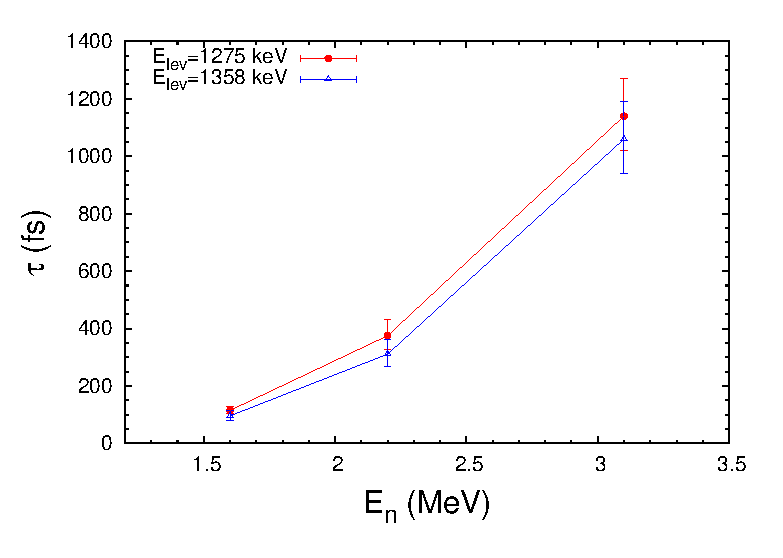
\includegraphics[width=0.85\textwidth]{figures/lifetime_inflation_example.eps}
\caption{Lifetime inflation of the measured lifetimes for two levels (E$_{lev}$=1275~keV and E$_{lev}$=1358~keV) in $^{162}$Dy caused by effects due to a higher bombarding neutron energy and unknown level-feeding from higher-lying states. \label{fig:lifetime_inflation}}
\end{center}
\end{figure}

For the interest of discussion in \S \ref{chp:discussion}, lifetimes are separated into smaller, more digestable tables based on their corresponding discussion sections (\textit{e.g.} a table containing lifetimes of 0$^+$ states, one for the 2$^+_\gamma$ band, etc). Unless otherwise noted, tables in this chapter will contain experimentally determined level energies, $\gamma$-ray energies, branching ratios measured from our angular distributions, multipole mixing fractions where applicable, and the lifetime of the state with applicable uncertainties for all of the above quantities.
%preface to results being listed in preparation for discussion, separated by 
\section{$^{160}$Gd Results}
Results from the $^{160}$Gd campaign were published in \cite{Lesher_160Gd0s}, where this work also outlines and reiterates the major results taken from the suite of experiments in \S \ref{sec:Gd_exp}. A level scheme outlining all measured lifetimes in the $^{160}$Gd campaign is shown in Figure \ref{fig:160Gd_All}, with previously existing literature lifetimes in blue and new lifetime measurements in red. Prior to the presented results in this work, Gadolinium-160 has a complete paucity of lifetime information as a whole (most notably for 0$^+$ bands and negative parity bands), and as such, we add 29 new lifetimes, a factor of 7 increase, to the pool of placed literature values.

\begin{landscape}
\begin{center}
\begin{figure}[h!]
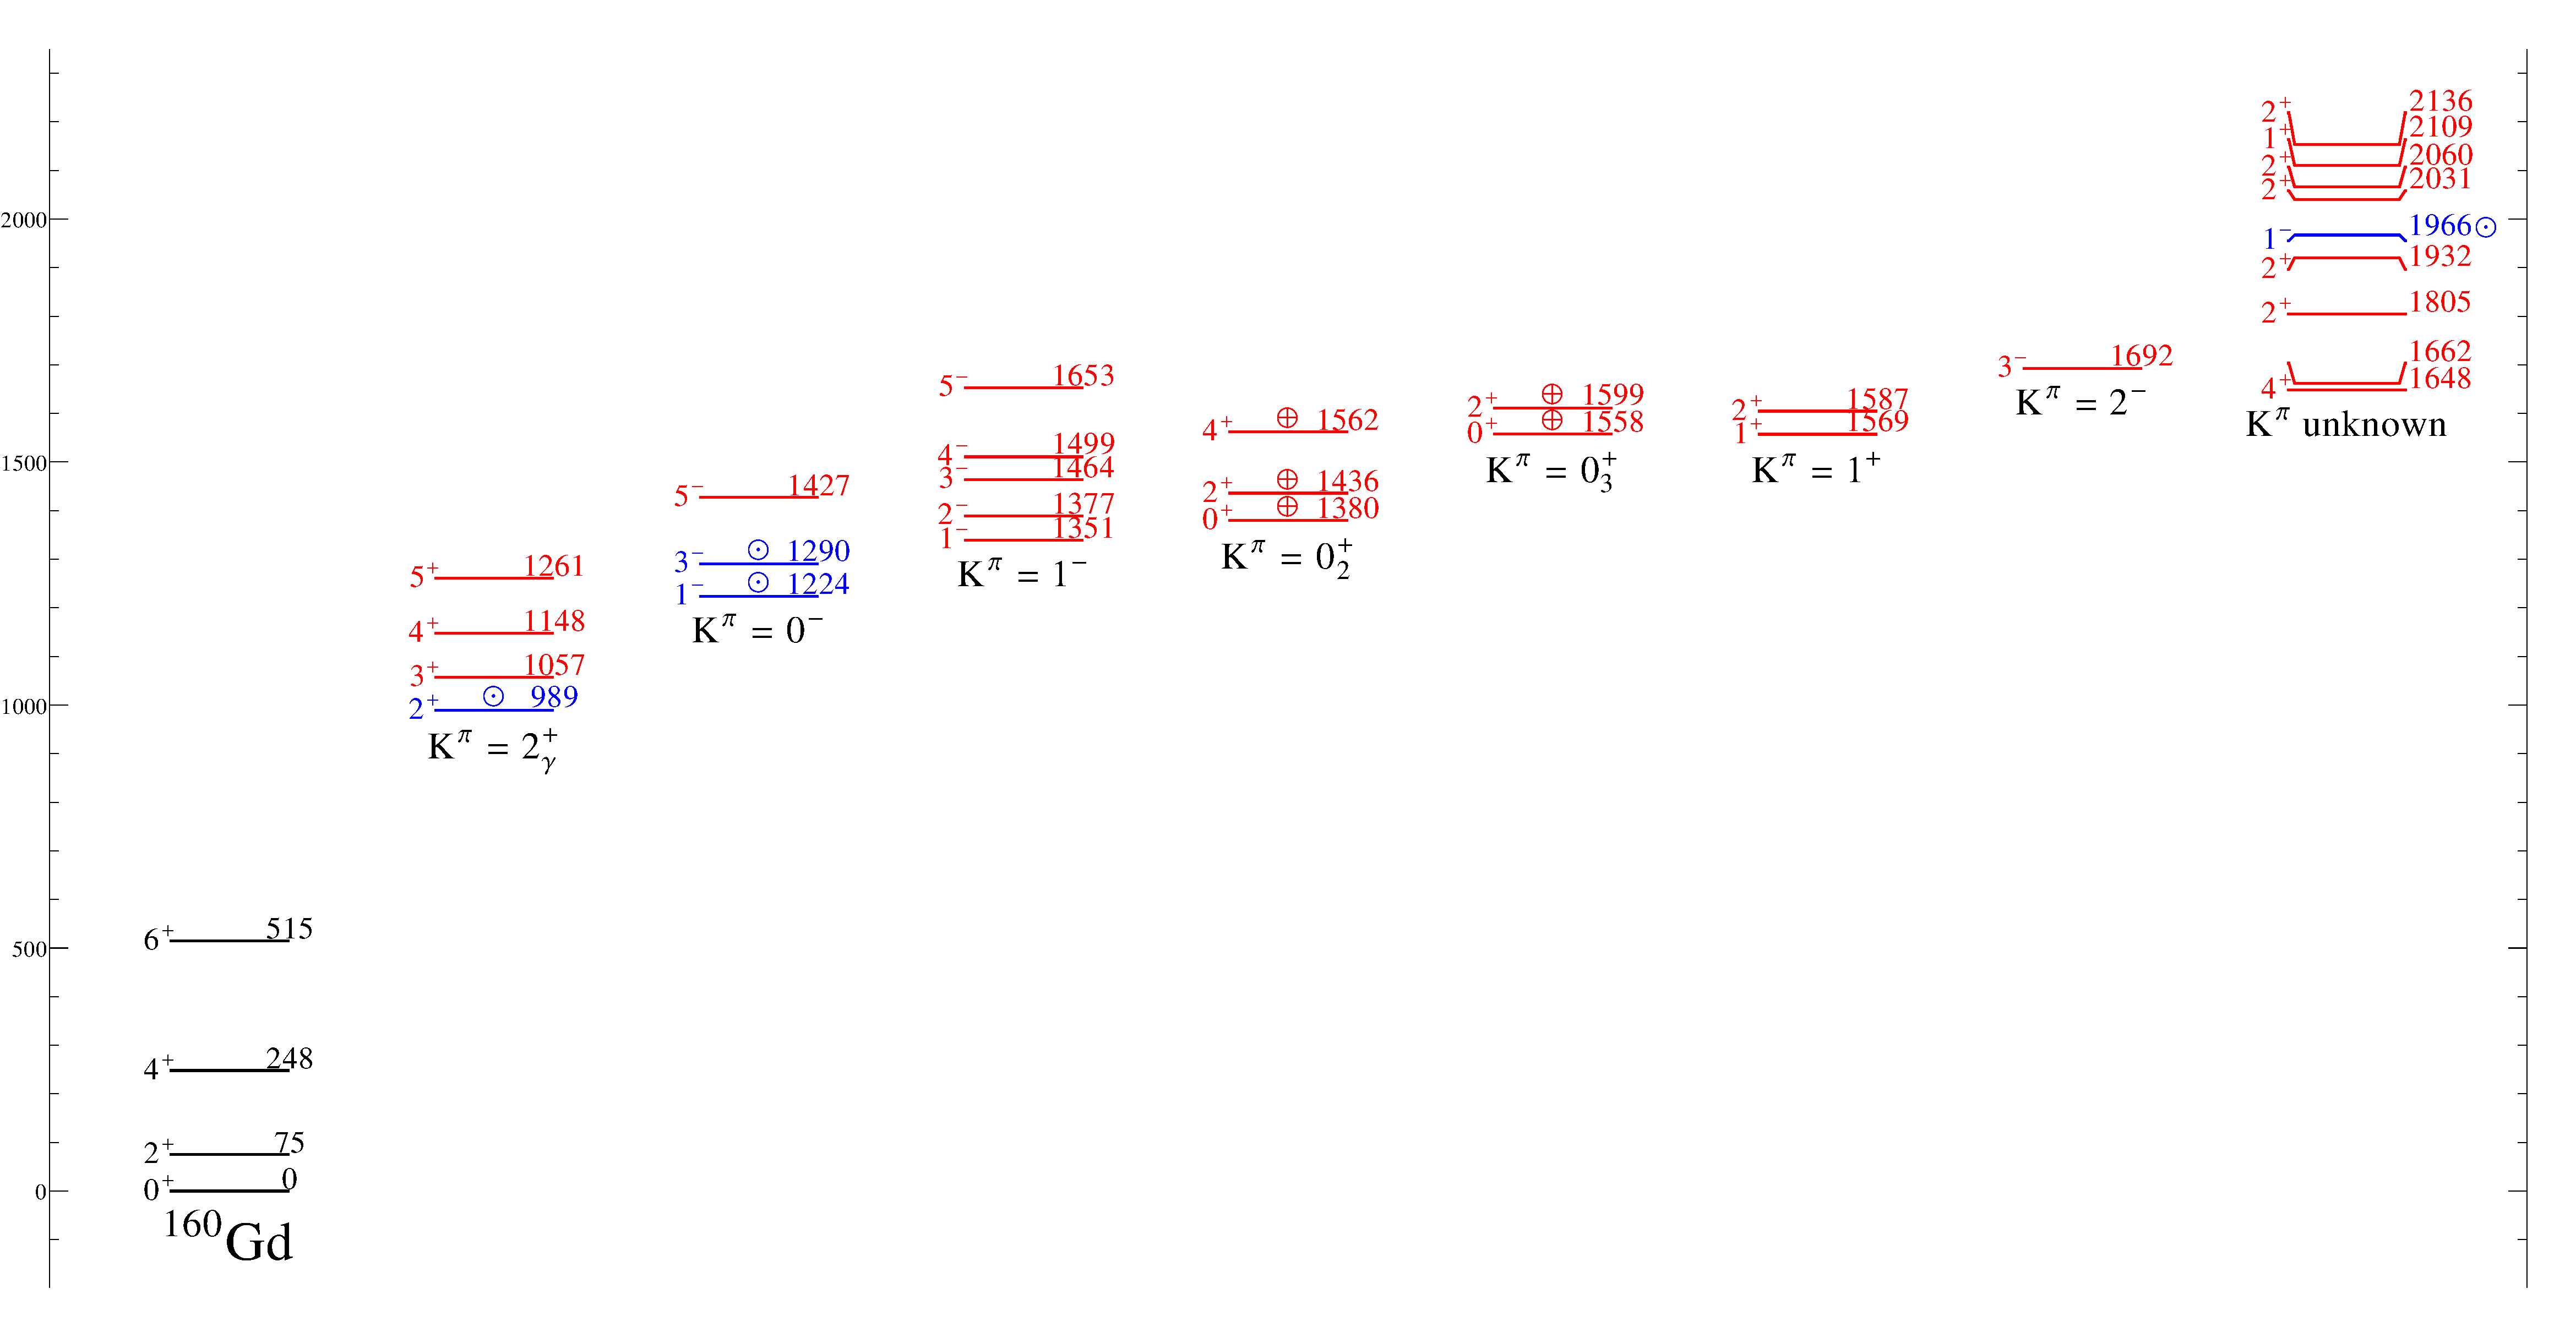
\includegraphics[height=0.85\textheight]{figures/160Gd_All.pdf}
\caption{Level scheme for all level lifetimes measured in the $^{160}$Gd experiments, with confirmed band and spin assignments shown. Previously measured lifetimes are in blue, with newly presented lifetimes in red. Individual levels and bands will be discussed in following sections.
\label{fig:160Gd_All}}
\end{figure}
\end{center}
\end{landscape}

High resolution angular distribution measurements were performed by Govor in \cite{Govor_160Gd_2009} and provide us with an overall benchmark for our measurements, and as a whole, our reported $\gamma$-ray intensities, angular distribution coefficients, and multipole mixing ratios are found to be in good agreement with the work. One key contrasted element in our work with the Govor paper is the use of monoenergetic neutrons for DSAM-INS rather than the continuum energies of reactor neutrons to extract the lifetimes in addition to any decay information ($\gamma$-ray energies, multipole mixing fractions, etc). A visual representation of the all the measured lifetimes in $^{160}$Gd is shown in Figure \ref{fig:160Gd_viz_lifetimes}, with literature values in black and new lifetimes in red (corresponding to lifetime extracted from the E$_n$=1.5~MeV dataset), green for 2.0~MeV neutrons, and blue for the final dataset using 2.8~MeV neutrons bombardement. %This figure also serves to show which bombarding neutron energies are used to extract level lifetimes (to minimize the inflation outlined as an example in Figure \ref{fig:lifetime_inflation}).

\begin{figure}[h!]
\begin{center}
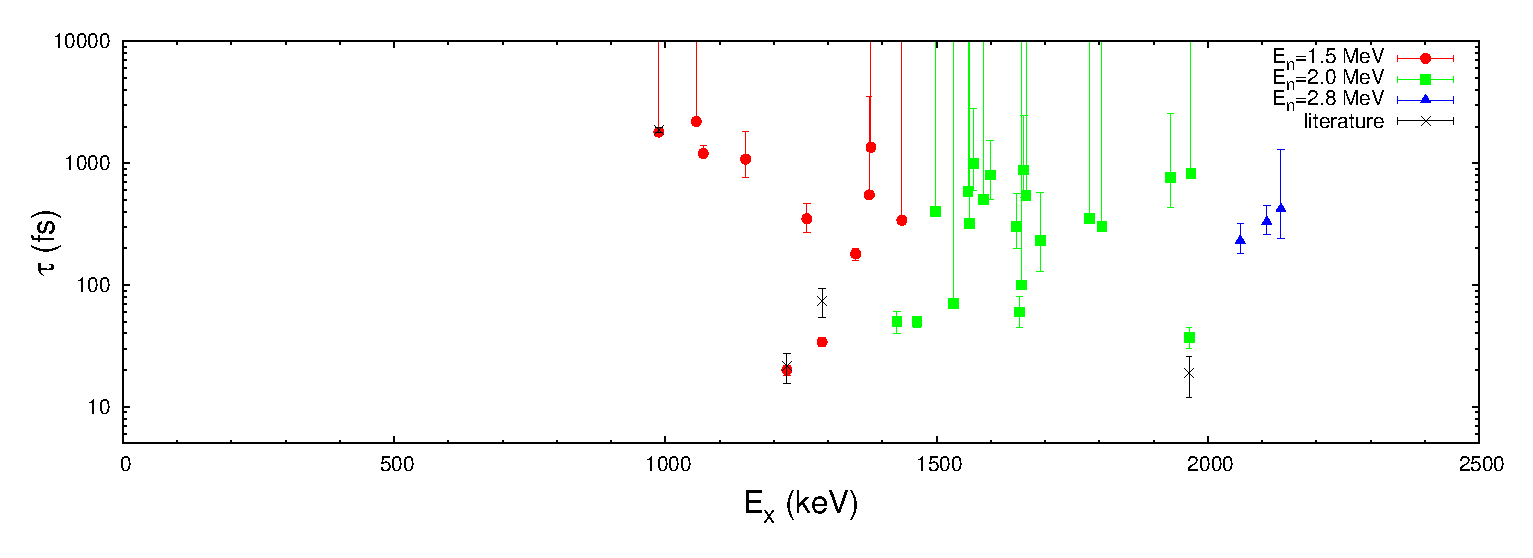
\includegraphics[width=0.95\textwidth]{figures/160Gd_viz_lifetimes.eps}
\caption{Visual representation of all measured lifetimes with respect to literature values (in blue). Each separate color outlines the specific regimes ($<$1.5~MeV, 1.5~-~2.0~MeV, and $>$2.0~MeV excitation energy) of energies studied in the $^{160}$Gd angular distributions. \label{fig:160Gd_viz_lifetimes}}
\end{center}
\end{figure}

An example of the E$_n$=2.0~MeV angular distribution singles-spectrum for $^{160}$Gd(n,n$^\prime\gamma$) can be seen in Figure \ref{fig:160Gd_200_spectrum} with select peaks labeled for reference.

\begin{figure}[h!]
\begin{center}
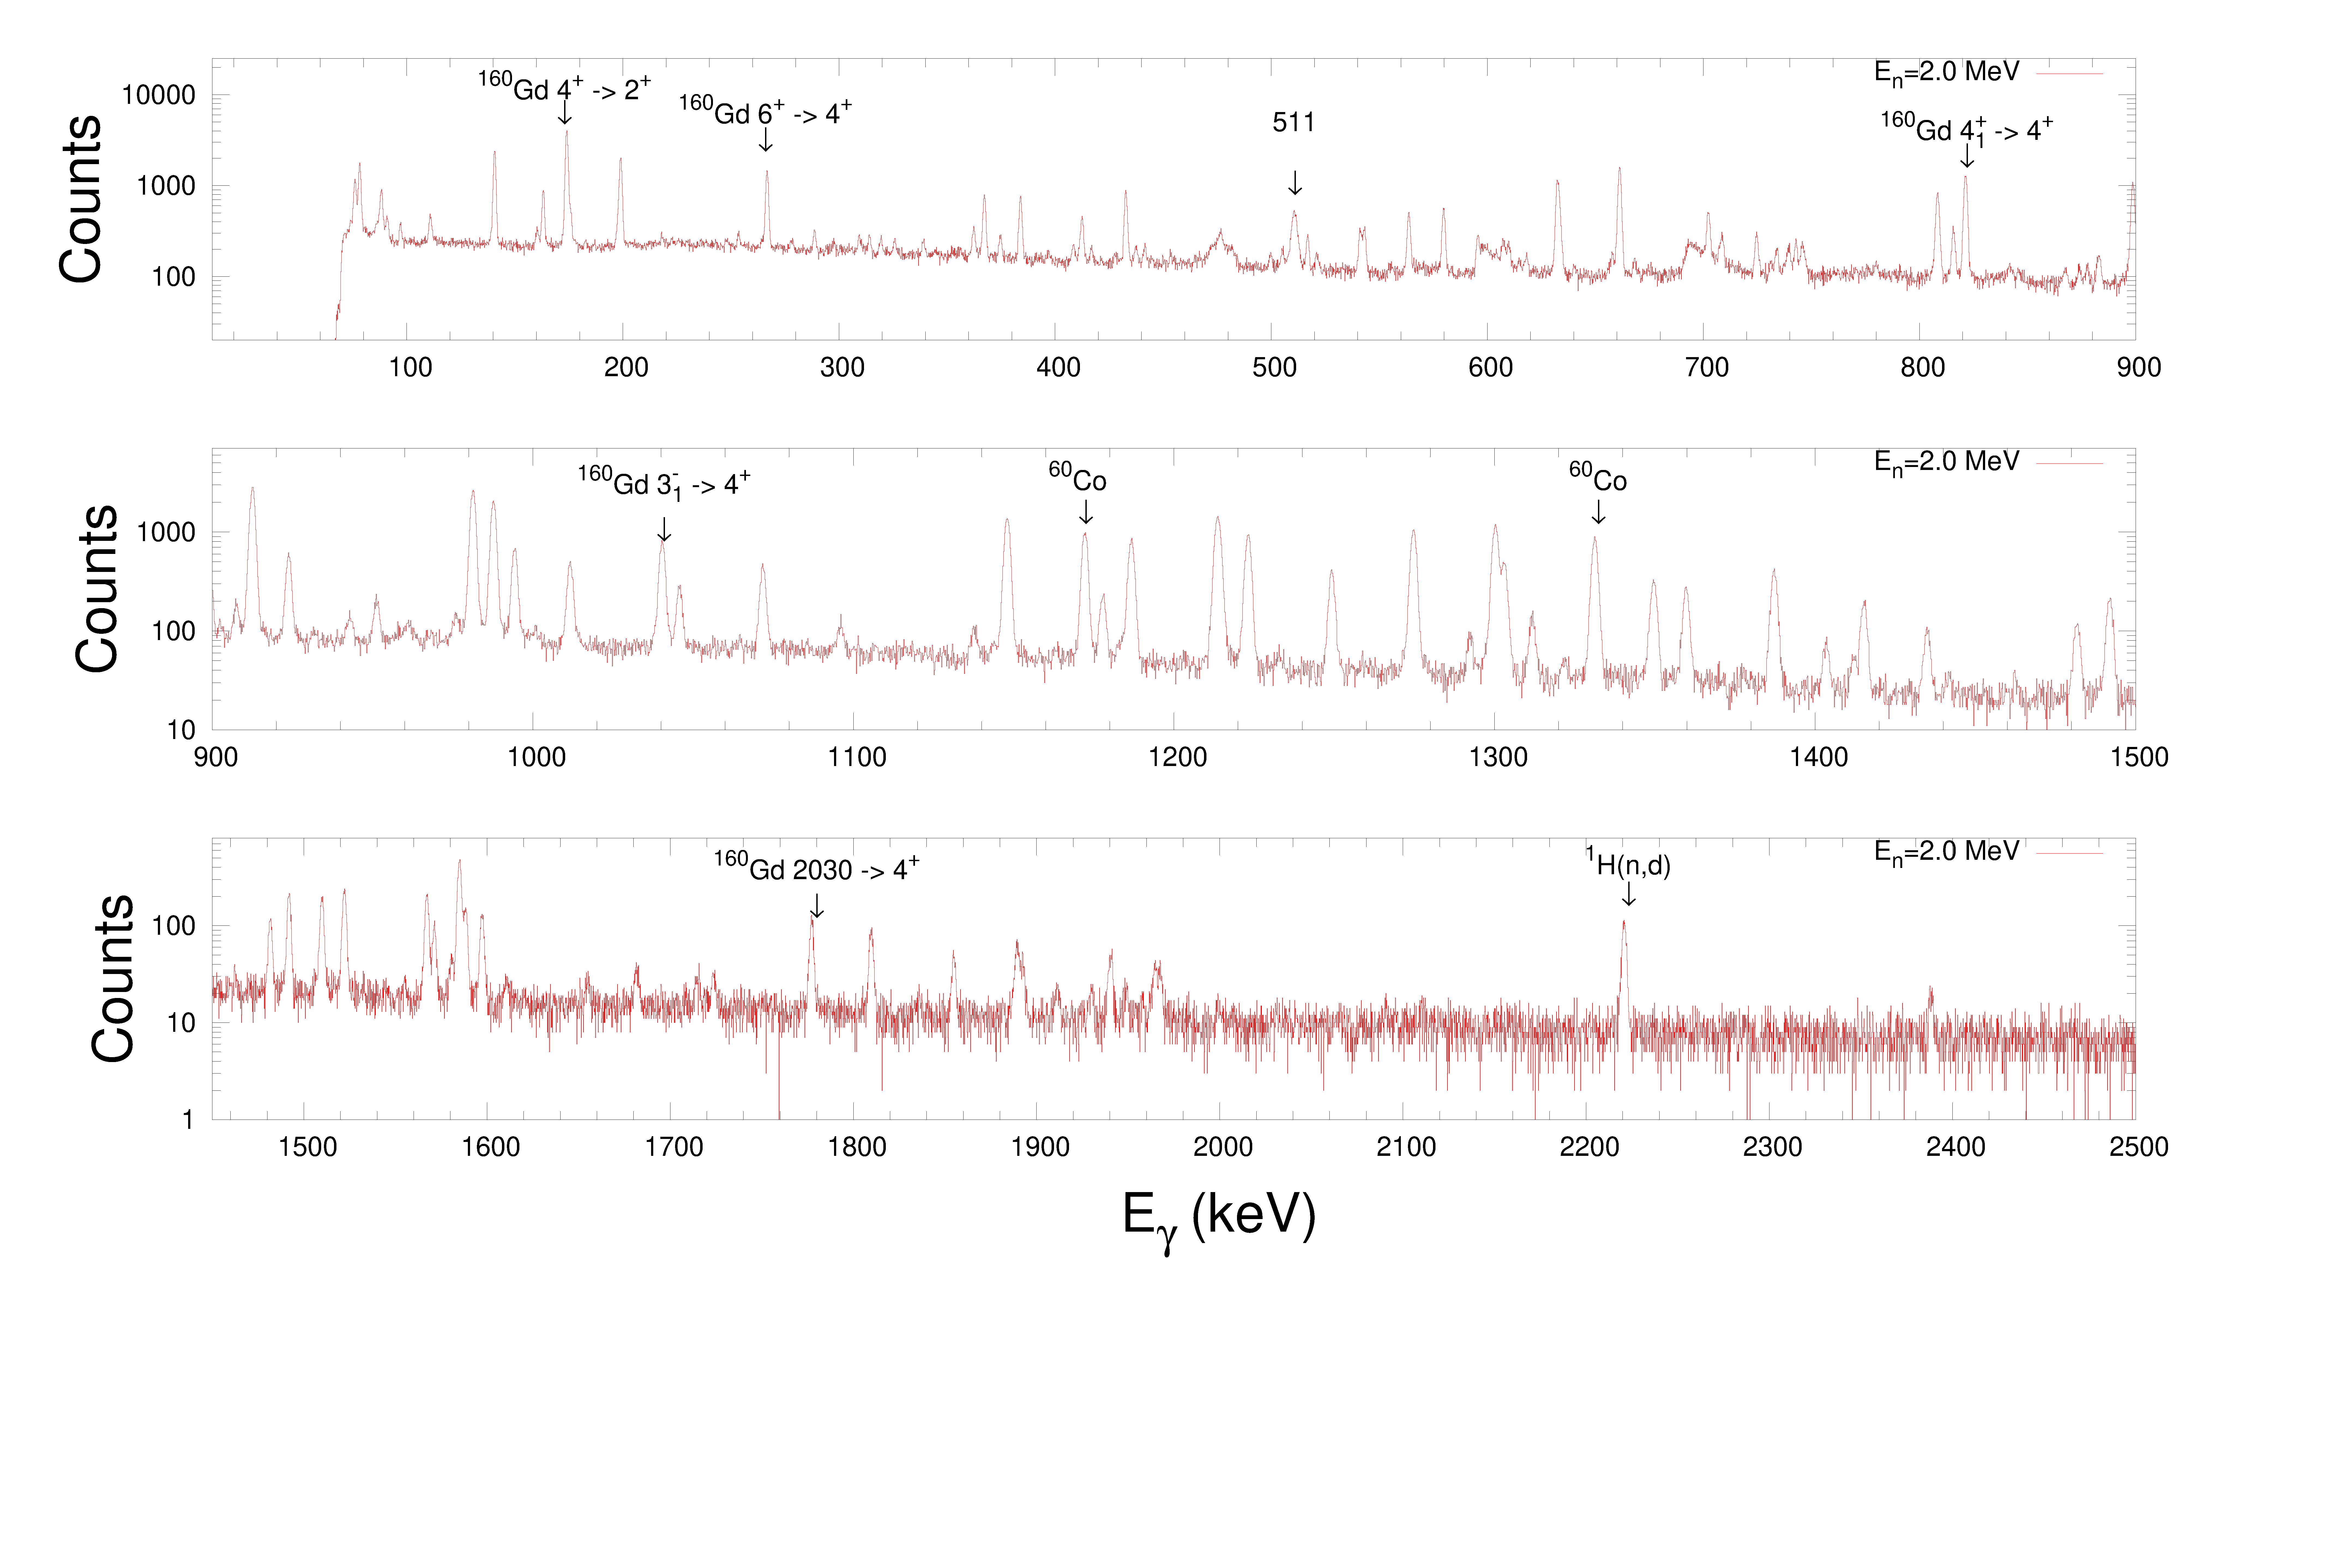
\includegraphics[width=0.95\textwidth]{figures/160Gd_200_spectra.eps}
\caption{Singles spectra from the $\theta_{lab}$=90$^\circ$ and E$_n$=2.0~MeV angular distributions of $^{160}$Gd. \label{fig:160Gd_200_spectrum}}
\end{center}
\end{figure}

% visualization and preface to results (overview)
\subsection{Lifetimes of 0$^+$ States}
%lifetimes of 0$^+$ states overview
The tabulation of lifetimes for the 0$^+$ bands in $^{160}$Gd is given in Table \ref{tab:160Gd_0s_all}. In many cases, F($\tau$) values for $\gamma$ rays were small, and as such, we are only able to extract lower limits for the level lifetimes. Further refinement of the level lifetime for the E$_{\rm x}$=1599~keV state was provided in [TBA REF], where any negative (and consequently impossible) F($\tau$) attenuation factors were removed from the weighted average for the level lifetime.

\begin{landscape}
\begin{table}[h!]
\begin{center}
\caption{K$^\pi$=0$^+$ BANDS: $^{160}$GD  \label{tab:160Gd_0s_all}}
% \makebox[\textwidth]{
\begin{tabular}{cccccccccc}
E$_{level}$ (keV) & E$_\gamma$ (keV) & J$^\pi_{K^\pi_i}$ & J$^\pi_{K^\pi_f}$ & $\tau$ (fs) & BR & Mult. &  B(E2) (W.u.) & B(E1) (mW.u.)\\
\hline
\hline
1379.70 (7) & 1304.46 (5) & 0$^+_{0^+_2}$ & 2$^+_{0^+_1}$ & $>$1350 & 1.000 & E2 & $<$3.10 & \\
1436.47 (4) & 1187.81 (5) & 2$^+_{0^+_2}$ & 4$^+_{0^+_1}$ & $>$340  & 0.667 & E2 & $<$13.1 & \\
            & 1361.05 (6) & 2$^+_{0^+_2}$ & 2$^+_{0^+_1}$ &         & 0.243 & E2/M1$^{[a]}$ & $<$2.42 & \\
            & 1436.34 (6) & 2$^+_{0^+_2}$ & 0$^+_{0^+_1}$ &         & 0.090 & E2 & $<$0.68 & \\
1561.59 (6) & 1046.67 (6) & 4$^+_{0^+_2}$ & 6$^+_{0^+_1}$ & $>$320  & 0.572 & E2 & $<$22 & \\
            & 1313.03 (6) & 4$^+_{0^+_2}$ & 4$^+_{0^+_1}$ &         & 0.428 & E2/M1$^{[b]}$ & $<$0.4 & \\   
            \hline
1558.30 (7) & 1483.06 (6) & 0$^+_{0^+_3}$ & 2$^+_{0^+_1}$ & $>$590  & 1.000 & E2 & $<$3.74 & \\
1599.00 (4) &  309.32 (6) & 2$^+_{0^+_3}$ & 3$^-_{0^-_1}$ & 800$^{+730}_{-300}$  & 0.037 & E1 &  & 0.34$^{+0.13}_{-0.31}$ \\
            &  374.78 (6) & 2$^+_{0^+_3}$ & 1$^-_{0^-_1}$ &              & 0.062 & E1 &  & 0.32$^{+0.12}_{-0.29}$ \\
            &  541.53 (6) & 2$^+_{0^+_3}$ & 3$^+_{2^+_\gamma}$ &         & 0.154 & E2/M1$^{[c]}$ & 41$^{+16}_{-37}$ & \\     
            & 1523.59 (6) & 2$^+_{0^+_3}$ & 2$^+_{0^+_1}$ &              & 0.418 & E2/M1$^{[d]}$ & 0.34$^{+0.68}_{-0.32}$ & \\
            & 1598.85 (6) & 2$^+_{0^+_3}$ & 0$^+_{0^+_1}$ &              & 0.329 & E2 & 0.41$^{+0.15}_{-0.37}$ & \\
            \hline

\end{tabular}\\ \vspace{10pt} \end{center}
% \begin{center}
Lifetimes of excited 0$^+$ bands in $^{160}$Gd, with experimentally determined B(E2) in W.u and B(E1) in mW.u.
$^{[a]}\delta$=0.00$^{+0.08}_{-0.08}$, $^{[b]}\delta$=0.28$^{+0.34}_{-0.12}$, $^{[c]}\delta$=-5.57$^{+1.91}_{-5.00}$, $^{[d]}\delta$=-1.04$^{+0.72}_{-2.10}$,%\\
1~W.u.(E2)=5.16E-7~e$^2$b$^2$, 1~mW.u.(E1)=1.90~e$^2$b\\
% \end{center}
\end{table}
\end{landscape}

\subsection{Lifetimes of 2$^+_\gamma$ Band}
%we have measured lifetimes in the gamma band yada yada
We have measured lifetimes for the 4 lowest-lying members of the K$^\pi$=2$^+$ band in $^{160}$Gd in our campaign of experiments. Throughout the rare-earth region of nuclei, the 2$^+$ band lifetimes are generally well known and fall in the near-picosecond lifetime range \cite{McGowan_BE2_1981,Burke_hexadecapole1994,PhysRevC.54.679,JAMMARI_1988}. Due to the sensitive range of DSAM, these near-picosecond lifetimes manifest as lower-limits due to the shallow F($\tau$) values observed in our experiments; however, we obtain well-defined values for the 4$^+$ and 5$^+$ members of the 2$^+$ band via some well-defined energy shifts, all shown in Table \ref{tab:160Gd_gamma}.

\begin{table}[h!]
\begin{center}
\caption{K$^\pi$=2$^+$ BAND: $^{160}$GD \label{tab:160Gd_gamma}}

\begin{tabular}{ccccccccc}
E$_{level}$ (keV) & E$_\gamma$ (keV) & J$^\pi_{K^\pi_i}$ & J$^\pi_{K^\pi_f}$ & $\tau$ (fs) & BR & Mult. &  B(E2) (W.u.) \\
\hline
\hline
988.72 (6)  & 913.43 (5) & 2$^+_{2^+_\gamma}$ & 2$^+_{0^+_{gs}}$ & $>$1800 & 0.530 & E2/M1$^{[a]}$ & $<$1.2\\%$^{+0.22}_{-0.18}$  \\ 
            & 988.68 (5) & 2$^+_{2^+_\gamma}$ & 0$^+_{0^+_{gs}}$ &         & 0.470 & E2         & $<$4.1\\%$^{+0.2}_{-0.2}$  \\ 

1057.42 (6) & 809.06 (5) & 3$^+_{2^+_\gamma}$ & 4$^+_{0^+_{gs}}$ & $>$2200 & 0.171 & E2/M1$^{[b]}$ & $<$0.04  \\ 
            & 982.28 (5) & 3$^+_{2^+_\gamma}$ & 2$^+_{0^+_{gs}}$ &         & 0.829 & E2/M1$^{[c]}$ & $<$6.5  \\ 

1148.15 (7) & 899.59 (5)  & 4$^+_{2^+_\gamma}$ & 4$^+_{0^+_{gs}}$ & 1080$^{+730}_{-320}$ & 0.631 & E2/M1$^{[d]}$ & 16$^{+5}_{-10}$  \\ 
            & 1072.85 (5) & 4$^+_{2^+_\gamma}$ & 2$^+_{0^+_{gs}}$ &                      & 0.369 & E2         & 3.8$^{+2.6}_{-1.1}$  \\ 

1261.24 (9) & 746.34 (5)  & 5$^+_{2^+_\gamma}$ & 6$^+_{0^+_{gs}}$ & 350$^{+120}_{-80}$ & 0.164 & E2/M1$^{[e]}$ & 31$^{+7}_{-11}$  \\ 
            & 1012.65 (5) & 5$^+_{2^+_\gamma}$ & 4$^+_{0^+_{gs}}$ &                    & 0.836 & E2/M1$^{[f]}$ & 35$^{+8}_{-12}$  \\ 
            \hline    
\end{tabular}\\ \vspace{10pt} \end{center}
Lifetimes of K$^\pi$=2$^+_\gamma$ band in $^{160}$Gd, with experimentally determined B(E2) in W.u. and multipole mixing fractions $\delta$ taken from the E$_n$=1.5~MeV angular distributions.
$^{[a]}\delta$=-0.45$^{+0.04}_{-0.05}$, $^{[b]}\delta$=0.11$^{+0.03}_{-0.03}$, $^{[c]}\delta$=47$^{+18}_{-10}$, $^{[d]}\delta$=21$^{+21}_{-7}$, $^{[e]}\delta$=8$^{+13}_{-4}$, $^{[f]}\delta$=15$^{+17}_{-6}$\\
1~W.u.(E2)=5.16E-7~e$^2$b$^2$\\
% \end{center}
\end{table}

\subsection{Lifetimes of Negative Parity Bands}

Population of the K$^\pi$=0$^-$ bands in rare-earth nuclei is abundant \cite{Zilges_K0dipole}, showing up as some of the strongest peaks in our $\gamma$-singles spectra, with a very low angular momentum transfer needed to populate the states ($\Delta$K=0). Typically, since the lowest-lying negative parity states are collective octupole vibrations on top of the deformed ground state, the mean lifetimes of these states are comparatively short, acting as a practical benchmark for lifetimes measurable by DSAM-INS. All three level lifetimes from the K$^\pi$=0$^-$ band in $^{160}$Gd were measured from the inelastic scatter of 1.5~MeV neutrons, using the five $\gamma$-rays listed in Table \ref{tab:160Gd_negparity}.

Similar to the K$^\pi$=0$^-$ band, the K$^\pi$=1$^-$ band in $^{160}$Gd is richly populated in our (n,n$^\prime\gamma$) experiments, with four band members (1$^-$,2$^-$,3$^-$,4$^-$) all proposed by Govor in another (n,n$^\prime\gamma$) study \cite{Govor_160Gd_2009} using continuum energy reactor neutrons in contrast to our monoenergetic probe. Of the specific lifetimes measured from the Doppler shifting $\gamma$-rays, we observe a weak decay from the 2$^-$ state to the $\gamma$-vibrational band; this branching ratio is so weak that it \textit{could} be misplaced, however, the threshold of the de-excitation in our excitation function does not place it leaving any other level. The resulting lifetime from the 1301~keV $\gamma$ ray is only a lower-limit due to the shallow F($\tau$) value.

Grigoriev \cite{Grigoriev2012} places a K$^\pi$=2$^-$ assignment on the band with the E$_{\rm x}$=1691 \& 1782~keV members that was tentatively either a 2$^-$ or 3$^-$. We adopt this 2$^-$ assignment from our observed $\gamma$-decay channels, even without the measurement or observation of the 2$^-$ bandhead in our data.

\begin{table}[h!]    
\begin{center}
\caption{NEGATIVE PARITY BANDS: $^{160}$GD \label{tab:160Gd_negparity}}
                            
% \makebox[\textwidth]{                           
\begin{tabular}{ccccccccc}
E$_{level}$ (keV) & E$_\gamma$ (keV) & J$^\pi_{K^\pi_i}$ & J$^\pi_{K^\pi_f}$ & $\tau$ (fs) & BR & Mult. &   B(E1) (mW.u.)\\
\hline
\hline
1224.33 (6)  & 1149.12 (5) & 1$^-_{0^-_1}$ & 2$^+_{0^+_1}$ & 20$^{+2}_{-2}$   & 0.597 & E1   & 6.5$^{+0.6}_{-0.6}$ &\\
             & 1224.38 (5) & 1$^-_{0^-_1}$ & 0$^+_{0^+_1}$ &                  & 0.403 & E1   & 3.6$^{+0.4}_{-0.4}$ &\\
1289.90 (7)  & 1041.37 (5) & 3$^-_{0^-_1}$ & 4$^+_{0^+_1}$ & 34$^{+3}_{-3}$   & 0.353 & E1   & 3.0$^{+0.3}_{-0.3}$ &\\
             & 1214.79 (5) & 3$^-_{0^-_1}$ & 2$^+_{0^+_1}$ &                  & 0.647 & E1   & 3.5$^{+0.3}_{-0.3}$ &\\
1427.40 (12) & 1214.79 (5) & 5$^-_{0^-_1}$ & 4$^+_{0^+_1}$ & 50$^{+10}_{-10}$ & 1.000 & E1   & 4.0$^{+0.8}_{-0.8}$ &\\
\hline
1351.30 (6)  & 1276.06 (5) & 1$^-_{1^-_1}$ & 2$^+_{0^+_1}$ & 180$^{+20}_{-20}$      & 0.833 & E1   & 0.74$^{+0.08}_{-0.08}$ &\\
             & 1351.30 (5) & 1$^-_{1^-_1}$ & 0$^+_{0^+_1}$ &                        & 0.167 & E1   & 0.12$^{+0.01}_{-0.01}$ &\\
1376.70 (8)  &  319.38 (6) & 2$^-_{1^-_1}$ & 3$^+_{2^+_\gamma}$ & $>$550            & 0.017 & E1   & $<$0.18 &\\
             & 1301.46 (5) & 2$^-_{1^-_1}$ & 2$^+_{0^+_1}$ &                        & 0.982 & E1   & $<$0.27 &\\
1464.00 (10) & 1388.75 (5) & 3$^-_{1^-_1}$ & 2$^+_{0^+_1}$ & 50$^{+5}_{-5}$         & 1.000 & E1  & 2.5$^{+0.2}_{-0.2}$ &\\
1498.94 (10) & 1250.39 (5) & 4$^-_{1^-_1}$ & 4$^+_{0^+_1}$ & $>$400                 & 1.000 & E1  & $<$0.41  &\\

\hline
1691.68 (7)  &  543.45 (6) & 3$^-_{2^-_1}$ & 4$^+_{2^+_\gamma}$ & 230$^{+350}_{-100}$ & 0.226 & E1   & 2$^{+1}_{-3}$ &\\
             &  634.56 (6) & 3$^-_{2^-_1}$ & 3$^+_{2^+_\gamma}$ &                     & 0.370 & E1   & 2.1$^{+0.9}_{-3.2}$ &\\
             &  702.84 (6) & 3$^-_{2^-_1}$ & 2$^+_{2^+_\gamma}$ &                     & 0.372 & E1   & 1.5$^{+0.7}_{-2.3}$ &\\
             & 1442.93 (8) & 3$^-_{2^-_1}$ & 4$^+_{0^+_1}$ &                          & 0.032 & E1   & 0.01$^{+0.01}_{-0.02}$ &\\
1782.67 (10) &  521.53 (8) & 4$^-_{2^-_1}$ & 5$^+_{2^+_\gamma}$ & $>$350              & 0.208 & E1   & $<$2.0 &\\
             &  725.19 (6) & 4$^-_{2^-_1}$ & 3$^+_{2^+_\gamma}$ &                     & 0.792 & E1   & $<$1.4 &\\
\end{tabular}\\ \vspace{10pt}
\end{center}
Lifetimes of excited negative parity bands in $^{160}$Gd, with experimentally determined B(E1) in mW.u. 
% 1~mW.u.(E1)=1.90~e$^2$b\\
\end{table}

\subsection{Lifetimes of Positive Parity Bands}
In addition to the measurement of lifetimes of K=0,2 and negative parity bands, we are also able to populate the vast majority of states below J=5. Lifetimes of positive parity bands were measured in $^{160}$Gd, namely of the K$^\pi$=4$^+$ and 1$^+$ bands. The full tabulation of measured lifetimes can be found in Table \ref{tab:160Gd_posparity}.


\begin{table}[h!]
\begin{center}
\caption{POSITIVE PARITY (K$^\pi$=4$^+$/1$^+$ BANDS): $^{160}$GD \label{tab:160Gd_posparity}}
\begin{tabular}{ccccccccc}
E$_{level}$ (keV) & E$_\gamma$ (keV) & J$^\pi_{K^\pi_i}$ & J$^\pi_{K^\pi_f}$ & $\tau$ (fs) & BR & Mult. &  B($\pi\ell$) \\
\hline
\hline
1070.57 (7) & 555.45 (8) & 4$^+_{4^+_1}$ & 6$^+_{0^+_1}$ & $>$1200  & 0.010 & E2            & $<$2.4  \\
            & 822.06 (5) & 4$^+_{4^+_1}$ & 4$^+_{0^+_1}$ &          & 0.603 & E2/M1$^{[a]}$ & $<$7.2  \\
            & 995.30 (5) & 4$^+_{4^+_1}$ & 2$^+_{0^+_1}$ &          & 0.387 & E2            & $<$5.2  \\
            \hline
1568.77 (6) & 217.51 (6)  & 1$^+_{1^+_1}$ & 1$^-_{1^-_1}$ & 1000$^{+1800}_{-400}$  & 0.030 & E1             & 0.97$^{+0.7}_{-1.8}$ \\
            & 580.20 (6)  & 1$^+_{1^+_1}$ & 2$^+_{2^+_\gamma}$ &                   & 0.305 & E2/M1$^{[b]}$  & 5.3$^{+6.7}_{-13}$  \\
            & 1493.40 (6) & 1$^+_{1^+_1}$ & 2$^+_{0^+_1}$ &                        & 0.323 & E2/M1$^{[c]}$  & 0.44$^{+0.23}_{-0.88}$  \\
            & 1568.70 (6) & 1$^+_{1^+_1}$ & 0$^+_{0^+_1}$ &                        & 0.342 & E2/M1$^{[*]}$  & 0.56$^{+0.22}_{-1.01}$  \\
1586.61 (12) & 1511.36 (6) & 2$^+_{1^+_1}$ & 2$^+_{0^+_1}$& $>$500                 & 1.000 & E2            & $<$4.01  \\
1665.16 (8) & 288.57 (6)  & 3$^+_{1^+_1}$ & 2$^-_{1^-_1}$ & $>$540                 & 0.115 & E1            & $<$2.9 \\
            & 1416.59 (6) & 3$^+_{1^+_1}$ & 4$^+_{0^+_1}$ &                        & 0.462 & E2/M1$^{[d]}$ & $<$0.73  \\
            & 1589.81 (6) & 3$^+_{1^+_1}$ & 2$^+_{0^+_1}$ &                        & 0.423 & E2/M1$^{[e]}$ & $<$0.95  \\
            \hline

\end{tabular}\\ \vspace{10pt}
\end{center}
% \begin{center}
Lifetimes of excited positive parity bands in $^{160}$Gd, with experimentally determined B(E2) in W.u and  B(E1) in mW.u. \\
$^{[a]}\delta$=-0.72$^{+0.06}_{-0.05}$, $^{[b]}\delta$=0.28$^{+0.25}_{-0.18}$, $^{[c]}\delta$=1.34$^{+1.6}_{-0.6}$, $^{[d]}\delta$=0.67$^{+0.11}_{-0.08}$, $^{[e]}\delta$=-1.87$^{+0.18}_{-0.18}$\\
$^{[*]}$ Full E2 strength is reported (no $\delta$ was calculated)\\
1~W.u.(E2)=5.16E-7~e$^2$b$^2$, 1~mW.u.(E1)=1.90~e$^2$b\\
% \end{center}
\end{table}

\subsection{Lifetimes of States with No K$^\pi$ Assignment}
The remaining lifetimes of states with no rotational band assignment are tabulated in Table \ref{tab:160Gd_Kunknown} and presented with deduced transition probabilities in Figure \ref{fig:160Gd_Kunknown}. We place stringent limits on the spin and parity of these states by confirming all de-excitations exhibit the same qualitative shape in the excitation functions, and by examining the Legendre polynomial coefficients to ascertain changes in angular momentum. In many cases, this is easily done if the radiation pattern is strongly E2 or E1; for mixed-multipolarity $\gamma$ rays, comparison to the {\tt CINDY} code is possible to restrict possible spin assignments. Generally, {\tt CINDY} is used as a baseline, rough assignment, as the statistical model behaves much better at lower mass nuclei, such as $^{76}$Ge or $^{106}$Pd \cite{Crider_76Ge_cindy,Peters2016_Pdshapecoex}, where the density of states above the pairing gap is smaller, and as such are tentative assignments placed by our (n,n$^\prime\gamma$) study.

% \begin{landscape}
\begin{table}[h!]
\begin{center}
\caption{OTHER LEVELS: $^{160}$GD \label{tab:160Gd_Kunknown}}

\begin{tabular}{ccccccccc}
E$_{level}$ (keV) & E$_\gamma$ (keV) & J$^\pi_{K^\pi_i}$ & J$^\pi_{K^\pi_f}$ & $\tau$ (fs) & BR & Mult. &  B($\pi\ell$) \\
\hline
\hline
1805.13 (9) & 734.50 (6)  & 2$^+_{[\Upsilon]}$ & 4$^+_{4^+_1}$ & $>$300   & 0.307 & E2                    & $<$76  \\
            & 816.46 (6)  & 2$^+_{[\Upsilon]}$ & 2$^+_{2^+_1}$ &          & 0.693 & E2/M1$^{[a]}$         & $<$37  \\\hline
1931.96 (7) &  874.51 (6) & 2$^+_{[\Upsilon]}$ & 3$^+_{2^+_1}$ & 760$^{+1800}_{-330}$  & 0.197 & E2/M1$^{[b]}$         & 8$^{+3.5}_{-19}$  \\
            & 1683.45 (7) & 2$^+_{[\Upsilon]}$ & 4$^+_{0^+_1}$ &                       & 0.206 & E2                    & 0.32$^{+0.14}_{-0.75}$  \\
            & 1856.65 (6) & 2$^+_{[\Upsilon]}$ & 2$^+_{0^+_1}$ &                       & 0.454 & E2/M1$^{[c]}$         & 0.20$^{+0.17}_{-0.47}$  \\
            & 1932.00 (7) & 2$^+_{[\Upsilon]}$ & 0$^+_{0^+_1}$ &                       & 0.143 & E2                    & 0.11$^{+0.05}_{-0.26}$  \\\hline
1966.66 (10)& 1891.33 (6) & 1$^+_{[\Upsilon]}$ & 2$^+_{0^+_1}$ & 37$^{+8}_{-7}$  & 0.637 & E1         & 0.84 $^{+0.28}_{-0.21}$  \\
            & 1966.97 (13)& 1$^+_{[\Upsilon]}$ & 0$^+_{0^+_1}$ &                 & 0.363 & E1         & 0.43 $^{+0.16}_{-0.11}$  \\\hline
1969.84 (9) & 1894.50 (6) & 2$^+_{[\Upsilon]}$ & 2$^+_{0^+_1}$ & $>$830   & 0.582 & E2/M1$^{[*]}$         & $<$0.45  \\
            & 1969.93 (7) & 2$^+_{[\Upsilon]}$ & 0$^+_{0^+_1}$ &          & 0.418 & E2                    & $<$0.27  \\\hline
2030.90 (9) & 1782.14 (6) & 2$^+_{[\Upsilon]}$ & 4$^+_{0^+_1}$ & $>$255   & 0.139 & E2/M1$^{[*]}$         & $<$0.47  \\
            & 1955.93 (7) & 2$^+_{[\Upsilon]}$ & 2$^+_{0^+_1}$ &          & 0.861 & E2                    & $<$1.84  \\\hline
2060.43 (11)& 2060.42 (6) & 2$^+_{[\Upsilon]}$ & 6$^+_{0^+_1}$ & 230$^{+90}_{-50}$  & 1.000 & E2         & 1.82 $^{+0.40}_{-0.71}$  \\\hline
2109.32 (7) & 1051.87 (6) & 1$^+_{[\Upsilon]}$ & 3$^+_{2^+_1}$ & 330$^{+120}_{-70}$   & 0.170 & E2                     & 6.23 $^{+1.34}_{-2.28}$ \\
            & 1119.71 (13)& 1$^+_{[\Upsilon]}$ & 2$^+_{2^+_1}$ &                     & 0.208 & E2/M1$^{[*]}$          & 5.57 $^{+1.21}_{-2.04}$ \\
            & 2034.26 (6) & 1$^+_{[\Upsilon]}$ & 2$^+_{0^+_1}$ &                      & 0.359 & E2/M1$^{[*]}$          & 0.49 $^{+0.10}_{-0.18}$ \\
            & 2109.31 (6) & 1$^+_{[\Upsilon]}$ & 0$^+_{0^+_1}$ &                      & 0.263 & E2/M1$^{[*]}$          & 0.30 $^{+0.06}_{-0.11}$ \\ \hline
2135.76 (13)& 2135.74 (7) & 2$^+_{[\Upsilon]}$ & 0$^+_{0^+_1}$ & 420$^{+880}_{-180}$  & 1.000 & E2         & 0.83 $^{+0.36}_{-1.75}$   \\

\end{tabular}\\ \vspace{10pt}
\end{center}
% \begin{center}
Lifetimes of excited states in $^{160}$Gd that have no K band assignment, with experimentally determined B(E2) in W.u and  B(E1) in mW.u. \\
$^{[a]}\delta$=-0.76$^{+0.10}_{-0.13}$, $^{[b]}\delta$=-3.3$^{+1.1}_{-2.4}$,  $^{[c]}\delta$=0.92$^{+0.41}_{-0.64}$\\
$^{[*]}$ Full E2 strength is reported (no $\delta$ was calculated)\\
1~W.u.(E2)=5.16E-7~e$^2$b$^2$, 1~mW.u.(E1)=1.90~e$^2$b\\
$[\Upsilon]$: No rotational K$^\pi$ band assignment given in literature.
% \end{center}
\end{table}
% \end{landscape}

% \subsection{Other (Intensity info)}
